\documentclass[12pt,a4paper]{article}

% 如果需要中文支持,推荐使用xeCJK + 字体设置
\usepackage{xeCJK}
\setCJKmainfont{SimSun}  % 示例:宋体,可根据系统字体情况更换
\usepackage{amsmath}      % 数学公式(如有需要)
\usepackage{graphicx}     % 插图
\usepackage{geometry}     % 调整页边距
\usepackage{fancyhdr}     % 自定义页眉页脚
\usepackage{indentfirst}  % 中文首行缩进
\usepackage{calc}         % 允许做长度运算(测量文字宽度等)
\usepackage{titlesec}
\usepackage{booktabs} % 解决 \midrule 和 \bottomrule 报错
\usepackage{enumitem} % 支持自定义列表格式
\usepackage{float}
\usepackage{subcaption}
\usepackage{tabularx}

% 设置 \section 级标题为:加粗、大字号(如 \Large)
\titleformat{\section}
	{\bfseries\large}    % 标题自身的格式
	{\thesection}        % 标题编号的显示方式
	{1em}                % 编号与标题文字之间的间距
	{}                   % 在标题文字前后可插入额外代码,此处为空
	
% 设置 \subsection 级标题为:加粗、中等字号(如 \normalsize)
\titleformat{\subsection}
	{\bfseries\normalsize}
	{\thesubsection}
	{1em}
{}

% 页面设置(可根据需要微调)
\geometry{
	left=2cm,
	right=2cm,
	top=1cm,
	bottom=1.5cm
}

% 不需要过大的行距,使用较接近单倍行距的设置
\renewcommand{\baselinestretch}{1}

% 仅在页脚居中显示页码,页眉保持为空
\pagestyle{fancy}
\fancyhf{}  % 清空默认的页眉页脚
\fancyfoot[C]{\thepage}
\renewcommand{\headrulewidth}{0pt}
\renewcommand{\footrulewidth}{0pt}

% 首行缩进2字符(中文习惯)
\setlength{\parindent}{0pt}
\setlength{\leftskip}{2em}

\begin{document}
	%-------------------------------------------------------
	% 1 并排两个minipage:左标题、右校徽
	%   - 0.65\textwidth + 0.35\textwidth = \textwidth
	%   - 如果校徽过大或过小,可改宽度,如 0.25\textwidth、0.3\textwidth 等
	%   - 如果想让标题更大,可将 \Huge 改成 \huge 或 \LARGE
	%-------------------------------------------------------
	\noindent
	\hspace{-2em}
	\begin{minipage}[c]{0.65\textwidth}
		\raggedright
		{\fontsize{40pt}{60pt}\selectfont 物理实验报告}
	\end{minipage}
	\begin{minipage}[c]{0.35\textwidth}
		\raggedleft
		% 强制把校徽拉大到 0.35\textwidth 宽度 (高度自动匹配)
		% 若想指定高度,可用 "height=3cm" 等. 二选一即可.
		
\includegraphics[width=\linewidth, trim={20cm 20cm 20cm 20cm}, clip]{university_logo.png}
	\end{minipage}

	\vspace{-1em}
	

	%下方画两条分割线,并在两线之间写学号、姓名、日期、时间
	
	\hrule
	\vspace{0.4em}
	\noindent
	\begin{tabular}{l l l l}
    学号:\underline{114514} & 姓名:\underline{SUSTech} &
    日期:\underline{2025/03/08} & 时间:\underline{周二下午}
	\end{tabular}
	\vspace{-0em}
	\par
	\hrule

	

	%正文示例

	
	\section{实验名称:切变模量的测量}
	
	\section{实验目的}
		利用扭摆法测量钢丝的切变模量。

	\section{实验仪器}
		扭摆(已装待测钢丝)、圆环、千分尺、游标卡尺、卷尺、电子天平、电子计时器

	\section{实验原理}
	\subsection{剪切形变与切变模量}

	当材料受到平行于其表面的力作用时,会发生剪切形变。切变模量 (G) 是衡量材料抵抗剪切形变能力的物理量,定义为剪切应力 ($\tau$) 与剪切应变 ($\gamma$) 的比值。
	\begin{equation}
    G = \frac{\tau}{\gamma}
	\end{equation}
	其中,剪切应力 $\tau = \frac{F}{A}$,剪切应变 $\gamma = \frac{\Delta l}{l}$

	\subsection{扭摆的形成与运动}
	将金属丝一端固定,另一端悬挂物体,构成扭摆。扭转金属丝一定角度后释放,金属丝会恢复到原来的位置,从而对悬挂的物体产生一个力矩作用,使物体来回转动.

	\subsection{恢复力矩与扭转角的关系}
	当扭转角度足够小,且金属丝形变处于弹性限度内时,内部力矩与角度成正比。
	考虑金属丝横截面上的剪切形变。在距离轴线 $\rho$ 处的剪切应变为:
	\begin{equation}
    \gamma = \frac{\rho\theta}{l}
	\end{equation}
	其中 $\theta$ 是扭转角,$l$ 是金属丝的长度。
	由于在弹性限度内,剪切应力与应变成正比:$\tau = G\gamma$。
	因此,相对轴线的单位面积的力矩为:$\tau\rho$。
	考虑整个横截面,金属丝内部的总力矩为:
	\begin{equation}
    M = \iint \tau\rho \times dS = \int_{0}^{R} G\frac{\rho\theta}{l} \rho \times 2\pi\rho d\rho = \frac{\pi R^4 G}{2l}\theta
	\end{equation}
	其中 R 是金属丝的半径。

	引入矢量符号,上述方程可写为:
	\begin{equation}
    M = -\frac{\pi R^4 G}{2l}\theta = -D\theta
	\end{equation}
	其中 D 被称为扭转常数。负号表示力矩的方向与角位移的方向相反。

	\begin{equation}
    D = \frac{\pi R^4 G}{2l}
	\end{equation}

	\subsection{扭摆的周期与切变模量}

	恢复力矩作用于悬挂的物体时,在忽略阻力的情况下,根据牛顿第二定律有:
	\begin{equation}
    I_0\frac{d^2\theta}{dt^2} + D\theta = 0
	\end{equation}
	这是一个简谐运动的方程。因此物体在恢复力矩作用下将会来回转动,周期为:
	\begin{equation}
    T_0 = 2\pi\sqrt{\frac{I_0}{D}}
	\end{equation}
	$I_0$ 为悬挂物体的转动惯量。

	为了消除悬挂物转动惯量 $I_0$ 的影响,实验中通过增加一个圆环来改变扭摆的转动惯量。加入圆环后的周期变为:
	\begin{equation}
    T_1 = 2\pi\sqrt{\frac{I_0 + I_1}{D}}
	\end{equation}
	$I_1 = \frac{1}{2}m(r_{in}^2 + r_{out}^2)$ 为圆环的转动惯量,m 为圆环的质量,$r_{in}$ 和 $r_{out}$ 分别为圆环的内外半径。

	联立上述两个周期公式,可以计算出扭转常数 D:
	\begin{equation}
    D = 4\pi^2\frac{I_1}{T_1^2 - T_0^2} = \frac{2\pi^2 m(r_{in}^2 + r_{out}^2)}{T_1^2 - T_0^2}
	\end{equation}

	由公式(5)可得,切变模量 G:
	\begin{equation}
    G = \frac{2l}{\pi R^4}D = \frac{4\pi lm(r_{in}^2 + r_{out}^2)}{R^4(T_1^2 - T_0^2)}
	\end{equation}


	\section{实验内容}
	\begin{enumerate}
		\item 测量几何参数:
		  \begin{itemize}
			\item 卷尺测量钢丝有效长度 $L$,各测 3 次取平均;
			\item 千分尺测量钢丝直径 $2r$,各测 3 次取平均;
			\item 游标卡尺测量圆环内外直径,各测 3 次取平均;
			\item 电子天平测量圆环质量;
		  \end{itemize}
		\item 测量扭摆周期:记录未装环和装环状态下的振动周期 $T_1$、$T_2$,每次计 10 周。
		\item 计算扭转常数D和切变模量G:采用国际单位制,计算钢丝的扭转常数与切变模量。以N.m/rad为单位,根据实验精度,保留4位有效数字。以GPa (1 GPa=$10^9$ Pa)为单位,保留3位有效数字。
		\item 不确定度分析:
		根据公式
			\begin{equation}
				\frac{\Delta G}{G} = \frac{\Delta l}{l} + \frac{\Delta m}{m} + \frac{2r_{\text{in}}\Delta r_{\text{in}}}{r_{\text{in}}^2+r_{\text{out}}^2} + \frac{2r_{\text{out}}\Delta r_{\text{out}}}{r_{\text{in}}^2+r_{\text{out}}^2} + \frac{4\Delta R}{R} + \frac{2T_1\Delta T_1}{T_1^2-T_0^2} + \frac{2T_0\Delta T_0}{T_1^2-T_0^2}\,. 
		  	\end{equation}
		  	\begin{itemize}
				\item 确定主要误差项:公式右边的每一项表示某个待测量对不确定度的贡献,分别计算每一项,进而确定主要误差项;
				\item 估算不确定度:本实验中,主要误差项相对于其他项大得多,因此取主要误差项。计算$\Delta G = \frac{\Delta G}{G} \times G$求出切变模量的不确定度 $\Delta G$。
				\item B类不确定度:$\Delta l = 1\,\text{mm},\quad \Delta m = 0.1\,\text{g},\quad \Delta r_{\text{in}} = \Delta r_{\text{out}} = 0.01\,\text{mm},\quad \Delta R = 0.002\,\text{mm},\quad \Delta T_0 = \Delta T_1 = \frac{\Delta t}{n},\quad \Delta t = 1\,\text{ms},\quad n = 10.$
		  	\end{itemize}
	  \end{enumerate}

	\section{数据记录}
	  根据实验原理及实验内容进行实验,并输入excel进行统计计算。

	\section{数据处理}
		\begin{figure}[htbp]
			\centering
			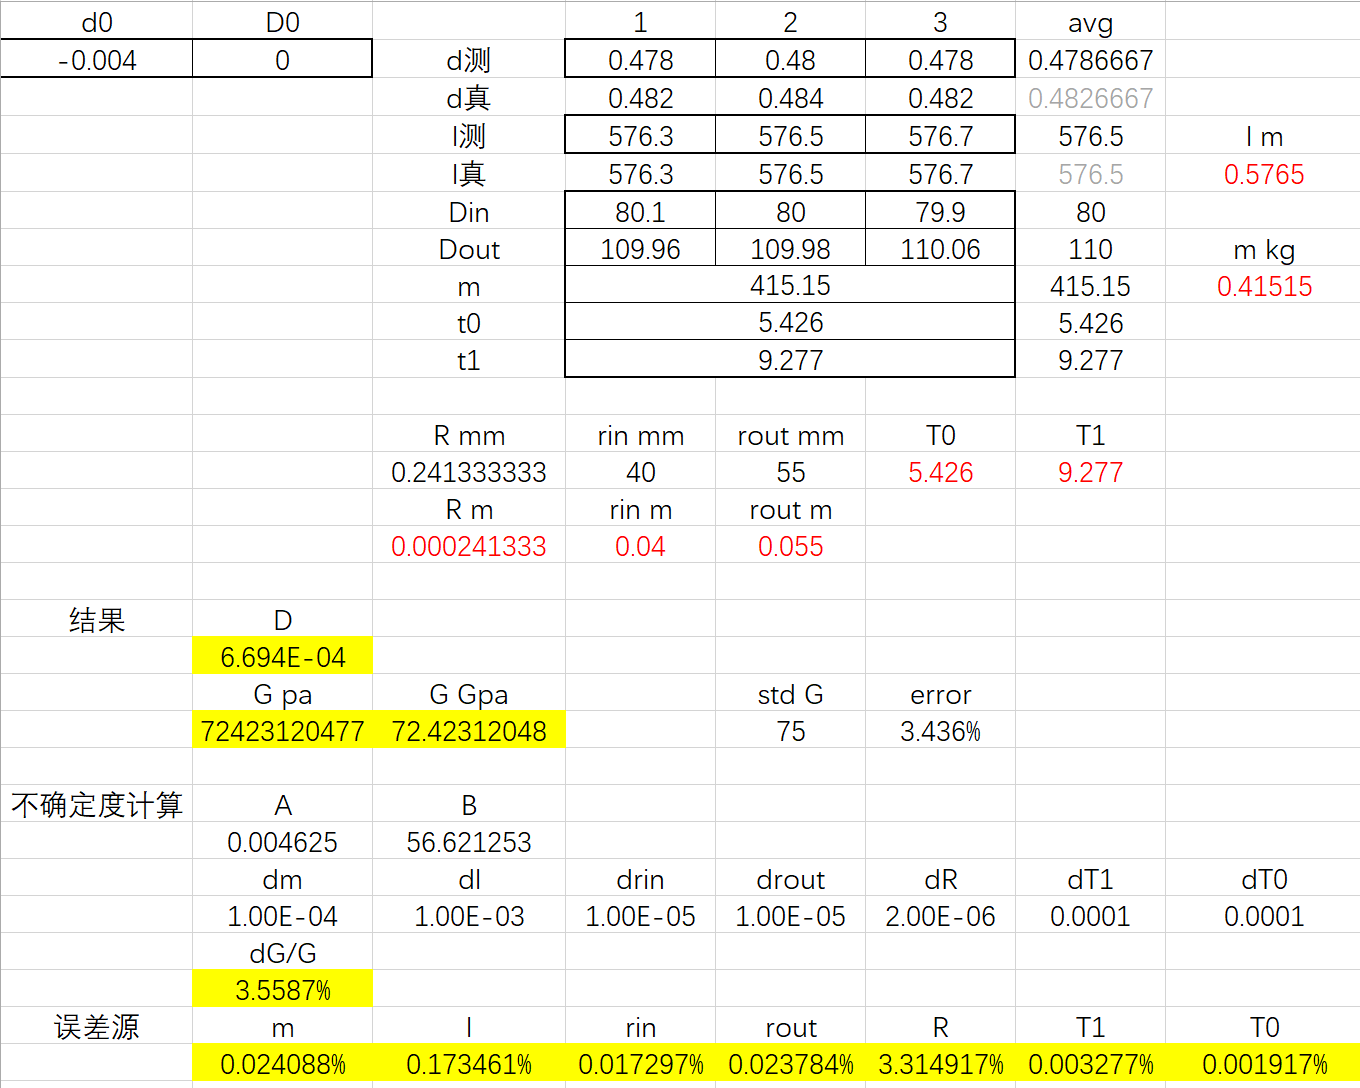
\includegraphics[width=0.6\textwidth]{数据处理.png}
			\caption{实验数据}
			\label{fig:数据}
	  	\end{figure}
	  	\subsection{计算平均值}
		根据excel计算,各个数据均值如下:\\
		\[
		l = 576.5\,\mathrm{mm}, R = 0.2413\,\mathrm{mm}, r_{\text{in}} = 40.00\,\mathrm{mm}, r_{\text{out}} = 55.00\,\mathrm{mm}, m = 415.15\,\mathrm{g}, T_0 = 5.426\,\mathrm{s}, T_1 = 9.277\,\mathrm{s}.
		\]
		\subsection{计算扭转常数 $D$}
		根据公式(9),代入数据计算可得$D = 6.694 \times 10^{-4}\,\mathrm{N\cdot m/rad}$
		\subsection{计算切变模量 $G$}
		根据公式(10),代入数据计算可得$G = 72.4\,\mathrm{GPa}$
	  	\subsection{估算不确定度}
			根据实验内容要求,计算各项不确定度,可得如下:
			\begin{itemize}
				\item $\frac{\Delta l}{l} \approx 0.173\% $
				\item $\frac{\Delta m}{m} \approx 0.024\% $
				\item $\frac{2r_{\text{in}}\Delta r_{\text{in}}}{r_{\text{in}}^2} \approx 0.017\%$
				\item $\frac{2r_{\text{out}}\Delta r_{\text{out}}}{r_{\text{in}}^2} \approx 0.024\%$
				\item $\frac{4\Delta R}{R} \approx 3.315\%$
				\item $\frac{2T_1\Delta T_1}{T_1^2-T_0^2} \approx 0.003\%$
				\item $\frac{2T_0\Delta T_0}{T_1^2-T_0^2} \approx 0.002\%$
			\end{itemize}
			可知,主要误差项源于R,再取主要误差项根据公式$\Delta G = \frac{\Delta G}{G} \times G$计算可得
			$\Delta G = \frac{\Delta G}{G} \times G \approx 2.4GPa$


	\section{实验结论}
	本实验利用扭摆法测量了钢丝的切变模量。通过测量钢丝的长度、直径,圆环的内外直径和质量,以及扭摆的周期,计算得到了钢丝的扭转常数和切变模量。\\
	扭转常数 $D = 6.694 \times 10^{-4}\,\mathrm{N\cdot m/rad}$ \qquad 切变模量 $G = (G \pm \Delta G) \approx (72.4\pm2.4) \,\text{GPa}$\\
	实验用304不锈钢切变模量的参考值为 74—77 GPa 且 72.4+2.4=74.8 GPa,故实验结果位于参考值区间,实验结果合理。\\
	实验误差来源:
	\begin{itemize}
		\item 测量过程中存在读数误差:例如测量钢丝长度时测量的是装好的仪器,不便读数导致误差较大
		\item 扭摆转动时不可避免存在上下振动,有非切向力,影响旋转周期
		\item 加圆环前后钢丝有一定形变,并非一直为定值
		\item 测量扭摆周期时时间计数器不一定位于平衡位置导致总时长有误差
	\end{itemize}	
	

\end{document}
